\documentclass[tikz,border=10pt]{standalone}
\usepackage{amsmath,amssymb}
\usetikzlibrary{calc,decorations.markings,arrows.meta,patterns,decorations.pathmorphing}
\usepgflibrary{fpu}

\definecolor{NavyDeep}{HTML}{0F172A}
\definecolor{BlueCore}{HTML}{1D4ED8}
\definecolor{BlueMid}{HTML}{3B82F6}
\definecolor{BlueLight}{HTML}{93C5FD}
\definecolor{TealAccent}{HTML}{0D9488}
\definecolor{TealLight}{HTML}{99F6E4}
\definecolor{OrangeAccent}{HTML}{D97706}
\definecolor{SlateGray}{HTML}{64748B}
\definecolor{SlateLight}{HTML}{F1F5F9}

\begin{document}
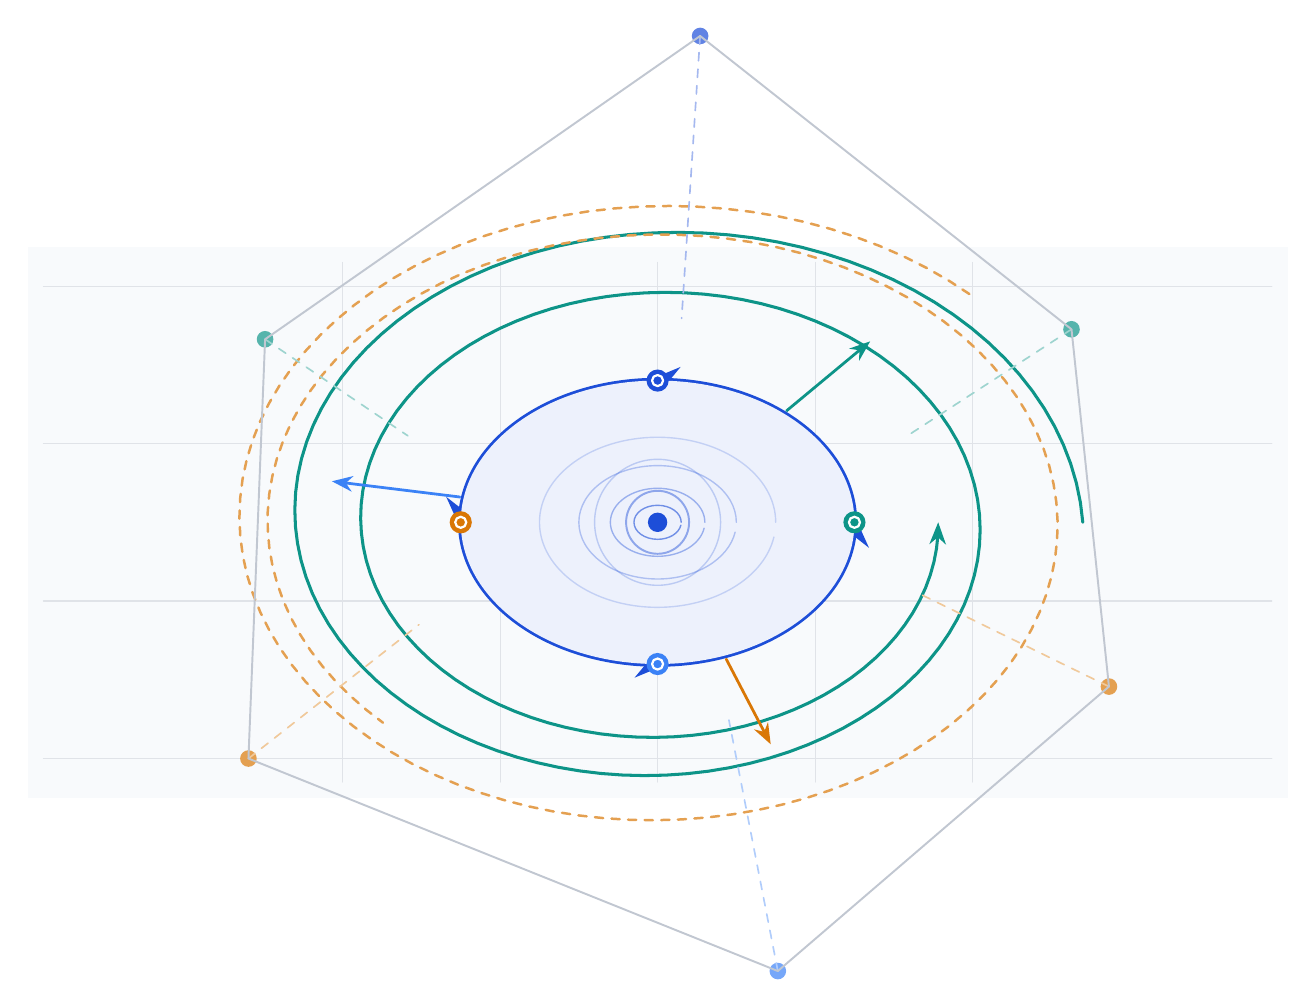
\begin{tikzpicture}[
  line cap=round, line join=round,
  >=Stealth,
  scale=1.0
]

% Background
\fill[SlateLight!50] (-8,-3.5) rectangle (8,3.5);

% === Inner loop: agent cognitive cycle (limit cycle in phase plane) ===
% Draw phase plane grid lightly
\foreach \x in {-4,-2,0,2,4} {
  \draw[SlateGray!20, line width=0.4pt] (\x,-3.3) -- (\x,3.3);
}
\foreach \y in {-3,-1,1,3} {
  \draw[SlateGray!20, line width=0.4pt] (-7.8,\y) -- (7.8,\y);
}

% The inner cognitive limit cycle (ellipse)
\draw[BlueCore, line width=2.0pt]
  (0,0) ellipse (2.5cm and 1.8cm);

% Arrow decorations on inner cycle (4 arrows)
\foreach \ang in {0,90,180,270} {
  \draw[BlueCore, line width=2.0pt, ->]
    ({2.5*cos(\ang+2)},{1.8*sin(\ang+2)}) -- ({2.5*cos(\ang+3)},{1.8*sin(\ang+3)});
}

% Fill inner cycle area
\fill[BlueCore!8] (0,0) ellipse (2.5cm and 1.8cm);

% Center attractor point
\fill[BlueCore] (0,0) circle (3.5pt);
\draw[BlueCore!50, line width=0.7pt] (0,0) circle (0.4cm);
\draw[BlueCore!30, line width=0.5pt] (0,0) circle (0.8cm);

% === Spiral trajectories converging TO the limit cycle from outside ===
% Outer spiral approaching the cycle
\draw[TealAccent, line width=1.1pt, ->]
  plot[domain=0:720, samples=200, variable=\t]
  ({(3.2+2.2*exp(-\t/400))*cos(\t)}, {(2.4+1.6*exp(-\t/400))*sin(\t)});

% Second outer spiral (rotated, dashed)
\draw[OrangeAccent!70, line width=0.9pt, dashed]
  plot[domain=0:540, samples=150, variable=\t]
  ({(4.8+0.8*exp(-\t/300))*cos(\t+45)}, {(3.5+0.6*exp(-\t/300))*sin(\t+45)});

% === External environment: scattered dots + connecting arrows to cycle ===
% Environment nodes (irregular polygon vertices)
\foreach \ang/\r/\col in {
  25/5.8/TealAccent,
  85/6.2/BlueCore,
  155/5.5/TealAccent,
  210/6.0/OrangeAccent,
  285/5.9/BlueMid,
  340/6.1/OrangeAccent%
}{
  \coordinate (env\ang) at ({\r*cos(\ang)}, {\r*sin(\ang)});
  \fill[\col!70] (env\ang) circle (3.0pt);
  % Draw line from env to edge of outer spiral
  \draw[\col!40, line width=0.6pt, dashed]
    (env\ang) -- ({3.5*cos(\ang)}, {2.6*sin(\ang)});
}

% Connect environment nodes with a polygon (knowledge/tool network)
\draw[SlateGray!40, line width=0.7pt]
  (env25) -- (env85) -- (env155) -- (env210) -- (env285) -- (env340) -- (env25);

% Radial "return" arrows from cycle edge back outward
\foreach \ang/\col in {50/TealAccent, 170/BlueMid, 290/OrangeAccent} {
  \draw[\col, line width=1.0pt, ->]
    ({2.55*cos(\ang)}, {1.85*sin(\ang)})
    -- ({4.2*cos(\ang)}, {3.0*sin(\ang)});
}

% === Fixed points / critical indicators on cycle ===
\foreach \ang/\col in {0/TealAccent, 90/BlueCore, 180/OrangeAccent, 270/BlueMid} {
  \fill[\col] ({2.5*cos(\ang)}, {1.8*sin(\ang)}) circle (4pt);
  \draw[white, line width=0.8pt] ({2.5*cos(\ang)}, {1.8*sin(\ang)}) circle (2pt);
}

% === Decorative: small phase trajectories inside the cycle ===
\foreach \r/\opa in {0.3/0.6, 0.6/0.4, 1.0/0.3, 1.5/0.2} {
  \draw[BlueCore, line width=0.5pt, opacity=\opa]
    ({2.5*\r/2.5},0) arc (0:350:{2.5*\r/2.5} and {1.8*\r/2.5});
}

\end{tikzpicture}
\end{document}
